\documentclass[11pt,a4paper]{article}
\usepackage[margin=1in]{geometry}
\usepackage{amsmath,amssymb,amsthm}
\usepackage{tikz}
\usepackage{pgfplots}
\pgfplotsset{compat=1.18}
\usepackage{graphicx}
\usepackage{xcolor}
\usepackage{enumitem}
\usepackage{hyperref}

\title{\textbf{Indifference Curves and Consumer Theory}\\ \large A Complete Guide}
\author{ECO 310 Midterm Review}
\date{}

\newtheorem{definition}{Definition}
\newtheorem{property}{Property}
\newtheorem{example}{Example}

\begin{document}

\maketitle

\tableofcontents
\newpage

\section{Introduction to Indifference Curves}

\begin{definition}[Indifference Curve]
An \textbf{indifference curve} is the set of all consumption bundles $(x_1, x_2)$ that provide the consumer with the same level of utility. Mathematically:
\[
IC_u = \{(x_1, x_2) : u(x_1, x_2) = \bar{u}\}
\]
where $\bar{u}$ is a constant utility level.
\end{definition}

The consumer is ``indifferent'' between any two points on the same indifference curve---they derive equal satisfaction from either bundle.

\subsection{Key Properties of Indifference Curves}

\begin{property}[Downward Sloping]
Indifference curves must slope downward (assuming both goods are desirable). To maintain constant utility, if you consume less of good 1, you must consume more of good 2 to compensate.
\end{property}

\begin{property}[Higher Curves = Greater Utility]
Indifference curves farther from the origin represent higher utility levels. This follows from the \textit{monotonicity} assumption: more is better.
\end{property}

\begin{property}[Never Cross]
Two indifference curves representing different utility levels can never intersect. If they did, the point of intersection would simultaneously represent two different utility levels, which is impossible.
\end{property}

\begin{property}[Convex to Origin]
For most preferences, indifference curves are convex (bowed inward toward the origin). This reflects \textit{diminishing marginal rate of substitution}.
\end{property}

\begin{center}
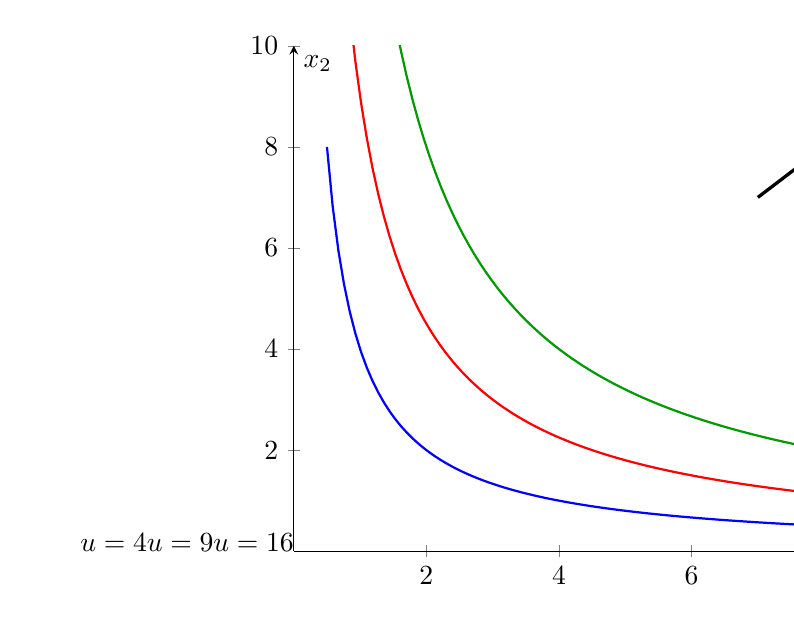
\begin{tikzpicture}
\begin{axis}[
    axis lines=middle,
    xlabel={$x_1$},
    ylabel={$x_2$},
    xmin=0, xmax=10,
    ymin=0, ymax=10,
    samples=100,
    domain=0.5:9,
    legend pos=north east,
    width=10cm,
    height=8cm
]

% Three indifference curves with u(x1,x2) = x1*x2
\addplot[blue, thick] {4/x};
\addlegendentryentry{$u = 4$}

\addplot[red, thick] {9/x};
\addlegendentryentry{$u = 9$}

\addplot[green!60!black, thick] {16/x};
\addlegendentryentry{$u = 16$}

% Arrow showing increasing utility
\draw[->, very thick] (axis cs:7,7) -- (axis cs:8.5,8.5) node[right] {Increasing Utility};

\end{axis}
\end{tikzpicture}
\end{center}

\section{Marginal Rate of Substitution (MRS)}

\begin{definition}[Marginal Rate of Substitution]
The \textbf{MRS} at a point is the rate at which a consumer is willing to substitute good 2 for good 1 while maintaining the same utility level. It equals the absolute value of the slope of the indifference curve:
\[
MRS_{12} = -\frac{dx_2}{dx_1}\bigg|_{u=\bar{u}}
\]
\end{definition}

\subsection{Computing MRS from Utility Functions}

For a utility function $u(x_1, x_2)$, the MRS can be calculated as:
\[
MRS_{12} = \frac{MU_1}{MU_2} = \frac{\partial u / \partial x_1}{\partial u / \partial x_2}
\]

\textbf{Derivation:} Along an indifference curve, utility is constant, so $du = 0$. Using total differential:
\begin{align*}
du &= \frac{\partial u}{\partial x_1}dx_1 + \frac{\partial u}{\partial x_2}dx_2 = 0\\
\frac{\partial u}{\partial x_1}dx_1 &= -\frac{\partial u}{\partial x_2}dx_2\\
\frac{dx_2}{dx_1} &= -\frac{\partial u / \partial x_1}{\partial u / \partial x_2} = -\frac{MU_1}{MU_2}
\end{align*}

Therefore: $MRS_{12} = \frac{MU_1}{MU_2}$

\begin{example}[Computing MRS]
For $u(x_1, x_2) = x_1^{1/2} x_2^{1/2}$:
\begin{align*}
MU_1 &= \frac{1}{2}x_1^{-1/2}x_2^{1/2} = \frac{1}{2}\sqrt{\frac{x_2}{x_1}}\\
MU_2 &= \frac{1}{2}x_1^{1/2}x_2^{-1/2} = \frac{1}{2}\sqrt{\frac{x_1}{x_2}}\\
MRS_{12} &= \frac{MU_1}{MU_2} = \frac{x_2}{x_1}
\end{align*}
\end{example}

\subsection{Diminishing MRS}

\textbf{Diminishing MRS} means that as you consume more of good 1 (moving right along an indifference curve), you're willing to give up less and less of good 2 for additional units of good 1.

\textbf{Economic Intuition:} The more you have of something, the less valuable an additional unit becomes relative to what you're giving up.

\textbf{Mathematical Implication:} For convex preferences, MRS decreases as $x_1$ increases along an indifference curve.

\section{Special Cases of Indifference Curves}

\subsection{Perfect Substitutes}

\textbf{Definition:} Goods are \textit{perfect substitutes} if the consumer is willing to substitute one for the other at a constant rate.

\textbf{Utility Function:} $u(x_1, x_2) = ax_1 + bx_2$ where $a, b > 0$

\textbf{MRS:} $MRS_{12} = \frac{a}{b}$ (constant)

\textbf{Indifference Curves:} Straight lines with slope $-a/b$

\begin{center}
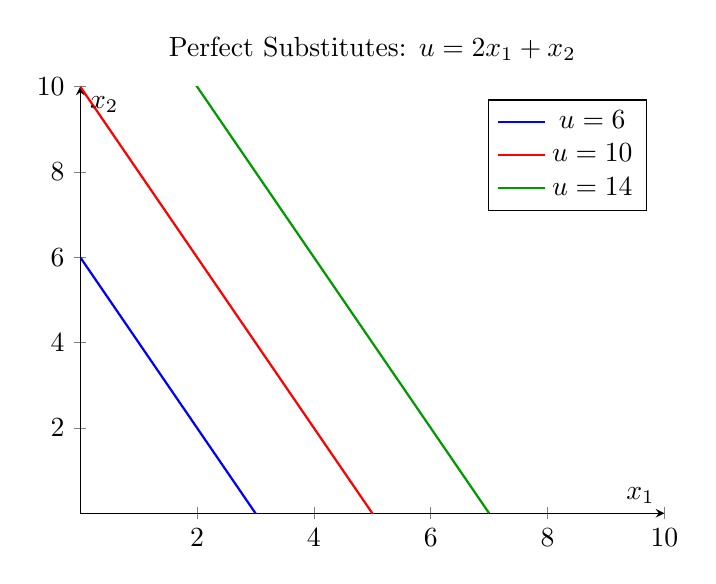
\begin{tikzpicture}
\begin{axis}[
    axis lines=middle,
    xlabel={$x_1$},
    ylabel={$x_2$},
    xmin=0, xmax=10,
    ymin=0, ymax=10,
    legend pos=north east,
    width=9cm,
    height=7cm,
    title={Perfect Substitutes: $u = 2x_1 + x_2$}
]

% Three parallel lines
\addplot[blue, thick, domain=0:10] {6 - 2*x};
\addlegendentry{$u = 6$}

\addplot[red, thick, domain=0:10] {10 - 2*x};
\addlegendentry{$u = 10$}

\addplot[green!60!black, thick, domain=0:7] {14 - 2*x};
\addlegendentry{$u = 14$}

\end{axis}
\end{tikzpicture}
\end{center}

\textbf{Example:} Nickels and dimes (2 nickels = 1 dime), different brands of identical products.

\subsection{Perfect Complements}

\textbf{Definition:} Goods are \textit{perfect complements} if they must be consumed in fixed proportions to provide utility.

\textbf{Utility Function:} $u(x_1, x_2) = \min\{ax_1, bx_2\}$ where $a, b > 0$

\textbf{MRS:} Undefined at the corner; $MRS = 0$ on horizontal segment, $MRS = \infty$ on vertical segment

\textbf{Indifference Curves:} L-shaped (right angles)

\begin{center}
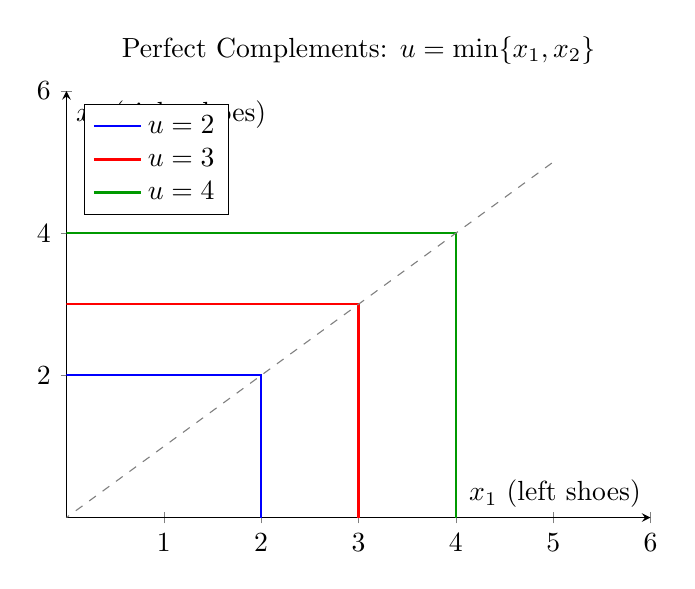
\begin{tikzpicture}
\begin{axis}[
    axis lines=middle,
    xlabel={$x_1$ (left shoes)},
    ylabel={$x_2$ (right shoes)},
    xmin=0, xmax=6,
    ymin=0, ymax=6,
    legend pos=north west,
    width=9cm,
    height=7cm,
    title={Perfect Complements: $u = \min\{x_1, x_2\}$}
]

% L-shaped curves
\addplot[blue, thick] coordinates {(0,2) (2,2) (2,0)};
\addlegendentry{$u = 2$}

\addplot[red, thick] coordinates {(0,3) (3,3) (3,0)};
\addlegendentry{$u = 3$}

\addplot[green!60!black, thick] coordinates {(0,4) (4,4) (4,0)};
\addlegendentry{$u = 4$}

% 45-degree line showing optimal consumption
\addplot[dashed, gray] {x};

\end{axis}
\end{tikzpicture}
\end{center}

\textbf{Example:} Left and right shoes, coffee and sugar (for some consumers), car engines and car bodies.

\subsection{Cobb-Douglas Preferences}

\textbf{Utility Function:} $u(x_1, x_2) = x_1^\alpha x_2^\beta$ where $\alpha, \beta > 0$

Often normalized so $\alpha + \beta = 1$: $u(x_1, x_2) = x_1^\alpha x_2^{1-\alpha}$

\textbf{MRS:}
\begin{align*}
MRS_{12} &= \frac{\alpha x_1^{\alpha-1}x_2^\beta}{\beta x_1^\alpha x_2^{\beta-1}} = \frac{\alpha}{\beta}\cdot\frac{x_2}{x_1}
\end{align*}

\textbf{Indifference Curves:} Smooth, convex hyperbolas (standard shape)

\begin{center}
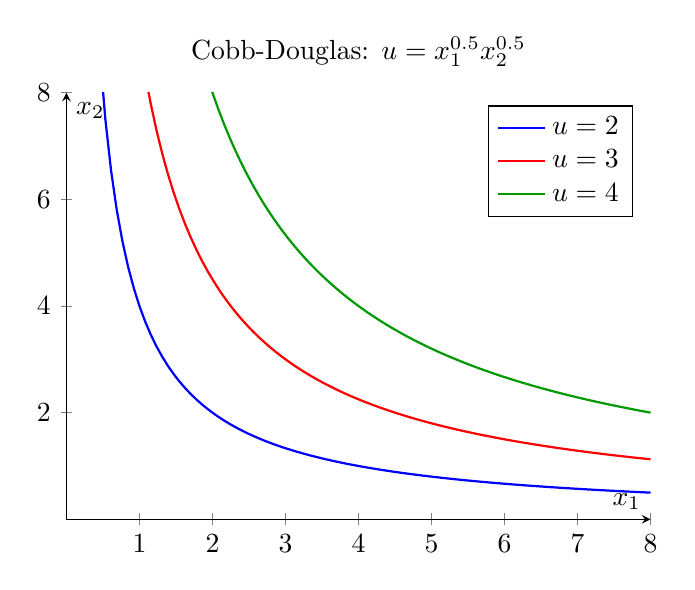
\begin{tikzpicture}
\begin{axis}[
    axis lines=middle,
    xlabel={$x_1$},
    ylabel={$x_2$},
    xmin=0, xmax=8,
    ymin=0, ymax=8,
    samples=100,
    domain=0.3:8,
    legend pos=north east,
    width=9cm,
    height=7cm,
    title={Cobb-Douglas: $u = x_1^{0.5} x_2^{0.5}$}
]

% Curves for u = x1^0.5 * x2^0.5
\addplot[blue, thick] {(2)^2/x};
\addlegendentry{$u = 2$}

\addplot[red, thick] {(3)^2/x};
\addlegendentry{$u = 3$}

\addplot[green!60!black, thick] {(4)^2/x};
\addlegendentry{$u = 4$}

\end{axis}
\end{tikzpicture}
\end{center}

\textbf{Key Property:} Constant expenditure shares! Consumer spends fixed fraction of income on each good:
\[
\frac{p_1 x_1}{m} = \frac{\alpha}{\alpha + \beta}, \quad \frac{p_2 x_2}{m} = \frac{\beta}{\alpha + \beta}
\]

\subsection{Quasilinear Preferences}

\textbf{Utility Function:} $u(x_1, x_2) = v(x_1) + x_2$ where $v$ is increasing and concave

\textbf{MRS:} $MRS_{12} = v'(x_1)$ (depends only on $x_1$, not $x_2$!)

\textbf{Indifference Curves:} Parallel vertical shifts of each other

\begin{center}
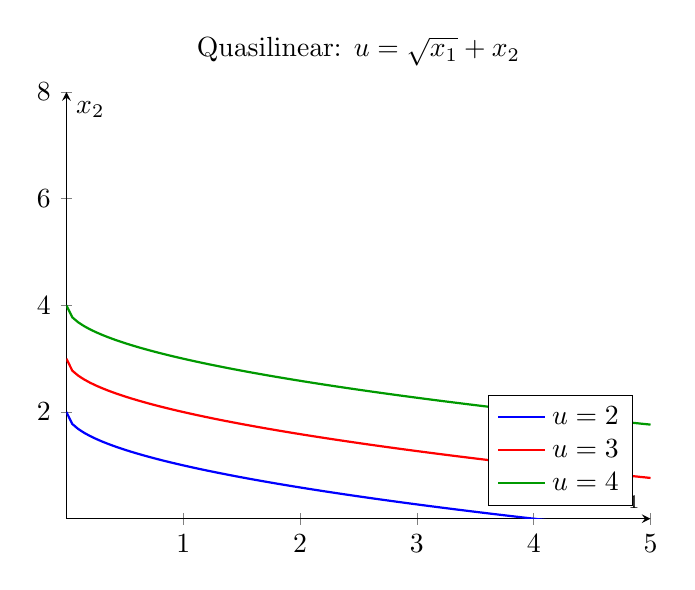
\begin{tikzpicture}
\begin{axis}[
    axis lines=middle,
    xlabel={$x_1$},
    ylabel={$x_2$},
    xmin=0, xmax=5,
    ymin=0, ymax=8,
    samples=100,
    domain=0:5,
    legend pos=south east,
    width=9cm,
    height=7cm,
    title={Quasilinear: $u = \sqrt{x_1} + x_2$}
]

% u = sqrt(x1) + x2, so x2 = u - sqrt(x1)
\addplot[blue, thick] {2 - sqrt(x)};
\addlegendentry{$u = 2$}

\addplot[red, thick] {3 - sqrt(x)};
\addlegendentry{$u = 3$}

\addplot[green!60!black, thick] {4 - sqrt(x)};
\addlegendentry{$u = 4$}

\end{axis}
\end{tikzpicture}
\end{center}

\textbf{Key Property:} No income effects for good 1! Demand for $x_1$ depends only on prices, not income.

\section{Consumer Optimization}

\subsection{Budget Constraint}

The budget line shows all affordable bundles:
\[
p_1 x_1 + p_2 x_2 = m
\]
where $m$ is income and $p_1, p_2$ are prices.

\textbf{Slope of budget line:} $-p_1/p_2$

\subsection{Optimal Choice}

\textbf{Tangency Condition:} At the optimal interior solution, the indifference curve is tangent to the budget line:
\[
MRS_{12} = \frac{p_1}{p_2}
\]

\textbf{Interpretation:} The rate at which the consumer is willing to trade goods (MRS) equals the rate at which the market allows trade (price ratio).

\textbf{Full Optimality Conditions:}
\begin{align}
\frac{MU_1}{MU_2} &= \frac{p_1}{p_2} \tag{Tangency}\\
p_1 x_1 + p_2 x_2 &= m \tag{Budget constraint}
\end{align}

\begin{center}
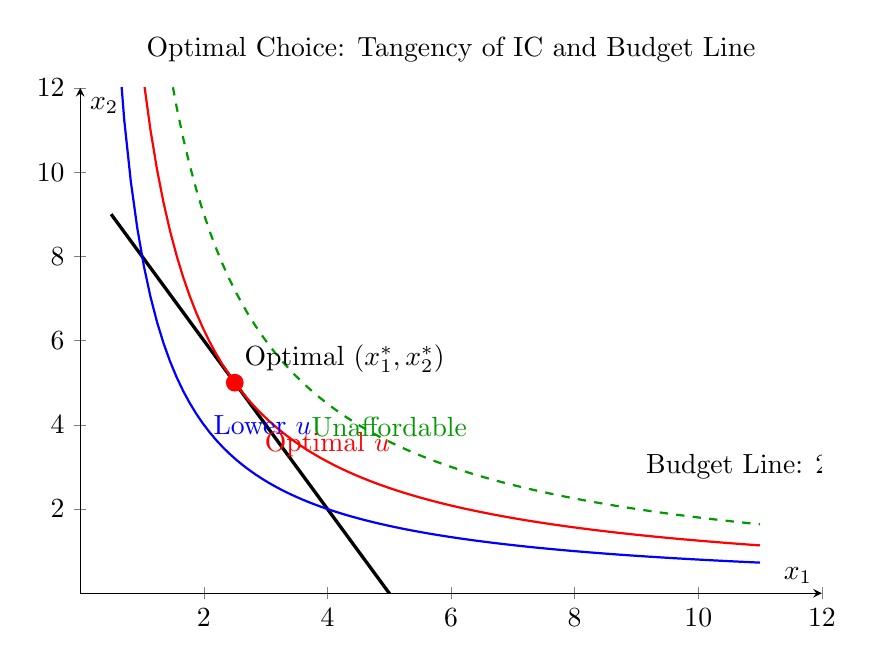
\begin{tikzpicture}
\begin{axis}[
    axis lines=middle,
    xlabel={$x_1$},
    ylabel={$x_2$},
    xmin=0, xmax=12,
    ymin=0, ymax=12,
    samples=100,
    domain=0.5:11,
    width=11cm,
    height=8cm,
    title={Optimal Choice: Tangency of IC and Budget Line}
]

% Budget line: 2x1 + x2 = 10
\addplot[black, very thick] {10 - 2*x};
\node at (axis cs:9,3) [right] {Budget Line: $2x_1 + x_2 = 10$};

% Indifference curves
\addplot[blue, thick] {8/x};
\addplot[red, thick] {12.5/x};
\addplot[green!60!black, thick, dashed] {18/x};

% Optimal point
\addplot[only marks, mark=*, mark size=3pt, red] coordinates {(2.5, 5)};
\node at (axis cs:2.5,5) [above right] {Optimal $(x_1^*, x_2^*)$};

% Lower utility (inside budget)
\node at (axis cs:2,4) [right, blue] {Lower $u$};
% Tangent utility
\node at (axis cs:4,3) [above, red] {Optimal $u$};
% Unaffordable
\node at (axis cs:5,3.5) [above, green!60!black] {Unaffordable};

\end{axis}
\end{tikzpicture}
\end{center}

\subsection{Corner Solutions}

Sometimes the optimal choice is on the boundary (consumer chooses zero of one good).

\textbf{Occurs when:} MRS $\neq$ price ratio even at the boundary.

\textbf{Example with Perfect Substitutes:} If $MRS = a/b < p_1/p_2$, consumer buys only good 2.

\begin{center}
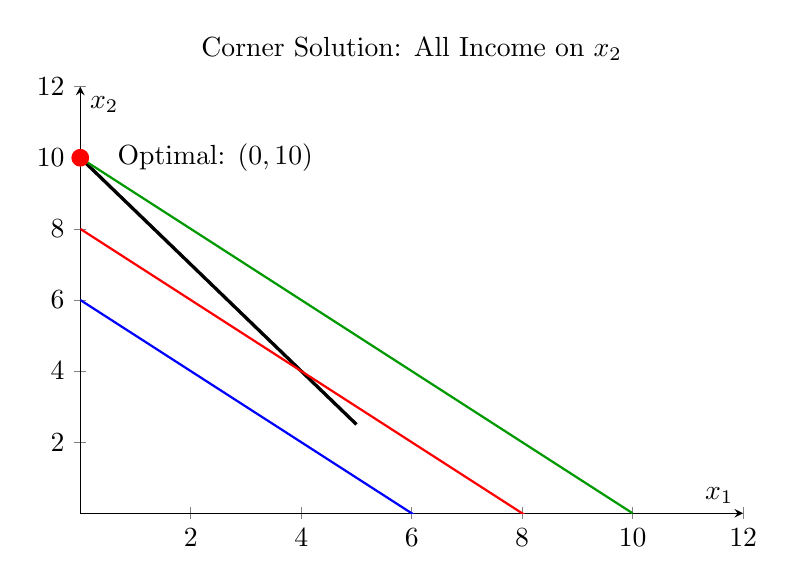
\begin{tikzpicture}
\begin{axis}[
    axis lines=middle,
    xlabel={$x_1$},
    ylabel={$x_2$},
    xmin=0, xmax=12,
    ymin=0, ymax=12,
    width=10cm,
    height=7cm,
    title={Corner Solution: All Income on $x_2$}
]

% Budget line
\addplot[black, very thick] {10 - 1.5*x};

% IC lines for perfect substitutes (slope = -1)
\addplot[blue, thick, domain=0:10] {6 - x};
\addplot[red, thick, domain=0:10] {8 - x};
\addplot[green!60!black, thick, domain=0:10] {10 - x};

% Optimal point at corner
\addplot[only marks, mark=*, mark size=3pt, red] coordinates {(0, 10)};
\node at (axis cs:0.5,10) [right] {Optimal: $(0, 10)$};

\end{axis}
\end{tikzpicture}
\end{center}

\section{Applications and Examples}

\subsection{Example 1: Deriving Demand (Cobb-Douglas)}

Given $u(x_1, x_2) = x_1^{1/3}x_2^{2/3}$, $p_1 = 2$, $p_2 = 1$, $m = 30$.

\textbf{Step 1: Tangency condition}
\begin{align*}
MRS &= \frac{p_1}{p_2}\\
\frac{(1/3)x_1^{-2/3}x_2^{2/3}}{(2/3)x_1^{1/3}x_2^{-1/3}} &= \frac{2}{1}\\
\frac{1}{2}\cdot\frac{x_2}{x_1} &= 2\\
x_2 &= 4x_1
\end{align*}

\textbf{Step 2: Budget constraint}
\begin{align*}
2x_1 + x_2 &= 30\\
2x_1 + 4x_1 &= 30\\
x_1 &= 5
\end{align*}

\textbf{Step 3: Solve for $x_2$}
\[
x_2 = 4(5) = 20
\]

\textbf{Answer:} Optimal bundle is $(x_1^*, x_2^*) = (5, 20)$.

\textbf{Check:} $\frac{p_1 x_1}{m} = \frac{2(5)}{30} = \frac{1}{3}$ $\checkmark$ (matches Cobb-Douglas exponent!)

\subsection{Example 2: Perfect Complements (Shoes)}

Given $u(L, R) = \min\{L, R\}$ (left and right shoes), $p_L = 1$, $p_R = 4$, $m = 10$.

\textbf{Key Insight:} Always consume in fixed ratio: $L = R$ (need equal numbers)

\textbf{Budget constraint with $L = R$:}
\begin{align*}
p_L L + p_R R &= m\\
1 \cdot L + 4 \cdot L &= 10\\
5L &= 10\\
L &= 2
\end{align*}

\textbf{Answer:} $(L^*, R^*) = (2, 2)$ — buy 2 pairs of shoes.

\textbf{Note:} If $p_R$ increases to 5:
- New budget: $L + 5L = 10 \Rightarrow L = 5/3$
- Demand for both decreases even though $p_L$ didn't change!
- This is the \textit{income effect}

\section{Summary: Convexity and MRS}

\begin{center}
\begin{tabular}{|l|c|c|c|}
\hline
\textbf{Preference Type} & \textbf{MRS} & \textbf{Shape} & \textbf{Convex?} \\
\hline
Perfect Substitutes & Constant & Straight line & Yes (weakly) \\
Perfect Complements & 0 or $\infty$ & L-shaped & Yes \\
Cobb-Douglas & $\frac{\alpha}{\beta}\frac{x_2}{x_1}$ & Smooth hyperbola & Yes \\
Quasilinear & $v'(x_1)$ & Parallel curves & Yes (if $v$ concave) \\
\hline
\end{tabular}
\end{center}

\textbf{Convex preferences} are standard and well-behaved:
\begin{itemize}
\item MRS is diminishing
\item Consumer prefers averages to extremes
\item Unique optimal interior solution (usually)
\end{itemize}

\textbf{When preferences are NOT convex:}
\begin{itemize}
\item MRS may be increasing
\item Consumer prefers extremes to averages
\item Multiple optimal solutions possible
\item Corner solutions more likely
\end{itemize}

\section{Quick Reference: Computing MRS}

\textbf{General Formula:}
\[
\boxed{MRS_{12} = \frac{MU_1}{MU_2} = \frac{\partial u/\partial x_1}{\partial u/\partial x_2}}
\]

\textbf{Common Utility Functions:}

\begin{enumerate}
\item \textbf{Cobb-Douglas:} $u = x_1^\alpha x_2^\beta$
\[
MRS = \frac{\alpha}{\beta}\cdot\frac{x_2}{x_1}
\]

\item \textbf{Perfect Substitutes:} $u = ax_1 + bx_2$
\[
MRS = \frac{a}{b}
\]

\item \textbf{Perfect Complements:} $u = \min\{ax_1, bx_2\}$
\[
MRS = \begin{cases} 0 & \text{if } ax_1 > bx_2\\ \infty & \text{if } ax_1 < bx_2\\ \text{undefined} & \text{if } ax_1 = bx_2 \end{cases}
\]

\item \textbf{Quasilinear:} $u = v(x_1) + x_2$
\[
MRS = v'(x_1)
\]

\item \textbf{CES:} $u = (x_1^\rho + x_2^\rho)^{1/\rho}$
\[
MRS = \left(\frac{x_2}{x_1}\right)^{1-\rho}
\]
\end{enumerate}

\end{document}
